\chapter{Analisi Formale}
Fino ad ora abbiamo analizzato i protocolli in maniera del tutto \textbf{informale}, utilizzando il linguaggio comune per ragionare sulla sicurezza di un protocollo. Chiaramente, l'analisi informale non basta per dimostrare che un protocollo è sicuro, poiché è soggetta a bias e dipende fortemente dall'esperienza di chi effettua l'analisi. 
Tuttavia, ci rendiamo conto che in realtà anche l'analisi informale ci può fornire qualche risultato. Di fatto, se troviamo un attacco dimostriamo chiaramente che il protocollo è insicuro nei confronti di quella specifica minaccia; tuttavia, se non lo troviamo, questo non basta a dimostrare che l'attacco non ci sia.

Vorremmo una sorta di strumento che ci dia garanzie formali riguardo alla \textbf{sicurezza} di un determinato protocollo \textbf{rispetto a una determinata proprietà}. La cosa più vicina a questo concetto che già conosciamo è la dimostrazione matematica, che certifica l'effettiva correttezza di un teorema. Queste dimostrazioni si basano su degli \textbf{assiomi} che vengono presi per veri e da cui si derivano altre verità. Possiamo dunque dire che la dimostrazione matematica non è altro che un \textbf{processo logico-deduttivo} che ci porta a dedurre ulteriori affermazioni vere, a patto che gli assiomi di partenza lo siano. Queste dimostrazioni sono \textbf{universali} e, dunque, non necessitano di un'enumerazione esaustiva di tutti i casi possibili per essere considerate valide.

Il nostro caso è però del tutto diverso: la sicurezza non è uno stato universale e, inoltre, non possiamo prendere per buoni assiomi assoluti. Quello che faremo noi sarà utilizzare un \textbf{modello finito} e definire la proprietà da ricercare come la \textbf{violazione della sicurezza} (ad esempio, la compromissione di una chiave). Infatti, se su questo modello riusciamo a dimostrare la presenza di una certa proprietà (ovvero troviamo l'attacco), allora possiamo affermare con certezza che questa vulnerabilità esiste anche nella generalizzazione del sistema. Tuttavia, \textbf{non è possibile dire che se una violazione non appare nel nostro modello finito, allora questa non esiste} nemmeno nel modello generalizzato.

Per quanto riguarda l'analisi formale, esistono diversi approcci, ognuno con le proprie peculiarità matematiche e concettuali:
\begin{itemize}
    \item \textbf{Algebre di processo (es. CSP, $\pi$-calculus):} Modellano i protocolli come sistemi di processi concorrenti. L'attenzione è posta sulla sequenza di eventi e sulle interazioni (sincronizzazioni) tra i vari agenti sui canali di comunicazione. Sono strumenti estremamente rigorosi per descrivere il parallelismo e il flusso dei dati.
    \item \textbf{Logiche di Autenticazione (es. BAN Logic):} Sono note come "logiche della credenza" (\textit{belief logics}). Invece di tracciare il singolo bit del messaggio, queste logiche modellano come evolve la conoscenza e la fiducia degli agenti passo dopo passo (ad esempio, formalizzando concetti come: "Se A riceve un messaggio cifrato con la chiave condivisa con B, allora A \textit{crede} che B lo abbia inviato"). Sono ottime per scovare assunzioni implicite ed errate sulla fiducia.
    \item \textbf{Linguaggi ad hoc (es. HLPSL):} Sono linguaggi di specifica creati appositamente per descrivere protocolli crittografici ad alto livello. Permettono di scrivere il protocollo in una sintassi vicina a quella umana (spesso derivata dalla notazione "Alice e Bob") per poi essere tradotti automaticamente in modelli matematici digeribili dai tool di analisi.
    \item \textbf{Dimostrazione automatica di teoremi (Theorem Proving, es. per induzione matematica):} Utilizza assistenti alla dimostrazione (come Isabelle/HOL o Coq) per applicare regole di inferenza logica, partendo dagli assiomi del sistema. Richiede un notevole sforzo manuale da parte dell'analista per guidare il software nella dimostrazione, ma offre la garanzia di correttezza universale per un numero illimitato di sessioni e agenti.
\end{itemize}
\section{Model Checking}
Il model checking è un metodo automatico per analizzare protocolli che mira non tanto a certificare la sicurezza assoluta, bensì a trovare degli attacchi (validazione per enumerazione). In pratica, specifichiamo il sistema target come una serie di \textbf{stati}, i quali possono essere interpretati come i fotogrammi di un video che rappresentano la configurazione del sistema in un dato istante. Lo stato può includere una rappresentazione epistemologica di ciò che conosce o può dedurre un determinato agente. Una volta generato lo spazio degli stati e fornita in input la proprietà da verificare, si procede ad un'analisi automatica tramite una macchina a stati finiti.

Più nel dettaglio, gli stati saranno generati secondo la sintassi di un certo linguaggio di modellazione, e la stessa cosa sarà fatta per la proprietà da verificare. Tuttavia, non è detto che i due linguaggi utilizzati coincidano. Spesso, infatti, risulta più comodo utilizzare linguaggi differenti (ad esempio, un linguaggio imperativo per definire le transizioni di stato e una \textit{logica temporale} per esprimere la proprietà desiderata).

I tool di model checking prendono in input il modello del protocollo e la proprietà da violare, per poi esplorare in automatico lo spazio degli stati. Questi strumenti enumerano tutti i possibili stati raggiungibili e verificano in ciascuno di essi se la proprietà si manifesta. 

La criticità principale di questo approccio è il cosiddetto problema della \textbf{state explosion} (esplosione dello spazio degli stati). Questo fenomeno si verifica quando le variabili, le sessioni parallele e le possibili azioni degli agenti generano un numero di stati che cresce in modo esponenziale (raggiungendo facilmente milioni o miliardi di combinazioni). In questi casi, il tool esaurisce la memoria o il tempo di calcolo prima di terminare l'enumerazione.

Se ci pensiamo, è anche logico che accada questo. Di fatto, analizzare un protocollo non vuol dire solamente andare a guardare i classici stati che vengono raggiunti poiché, sebbene il protocollo sia finito, in realtà ci sono molte fonti di infinitezza quando analizziamo un protocollo:
\begin{itemize}
    \item Potrebbero esserci \textbf{infiniti messaggi};
    \item I messaggi potrebbero essere \textbf{infinitamente lunghi};
    \item Possono esserci praticamente \textbf{infiniti agenti} ad eseguire il protocollo;
    \item L'attaccante potrebbe essere \textbf{infinitamente potente}.
\end{itemize}
Tutte queste fonti di infinitezza ci fanno capire chiaramente come un modello finito non sia abbastanza potente per poter effettuare l'analisi di un protocollo.
\section{Theorem Proving}
Come già accennato, le metodologie basate sulla dimostrazione di teoremi mirano a dare una prova di correttezza universale, evitando l'enumerazione degli stati come il model checking. 

In questo ambito si fa spesso uso della cosiddetta \textbf{dimostrazione per induzione}. In breve, la dimostrazione per induzione si applica a \textbf{insiemi definiti in modo induttivo}, come l'insieme dei numeri naturali $N$:
\begin{itemize}
    \item $0 \in N$
    \item Se $n \in N$, allora $succ(n) \in N$
\end{itemize}
Sulla base di questa struttura, possiamo definire il principio di induzione matematica per dimostrare una proprietà $P(n)$:
\begin{itemize}
    \item \textbf{Caso base:} Si dimostra che $P(0)$ è vera.
    \item \textbf{Passo induttivo:} Si assume che $P(n)$ sia vera (ipotesi induttiva) e si dimostra che $P(n) \implies P(succ(n))$.  
    \item \textbf{Conclusione:} Date queste precondizioni, possiamo affermare che la proprietà è universalmente valida: $\forall n \in N, P(n) = Vero$.
\end{itemize}
Grazie al metodo induttivo, possiamo dimostrare che valgono certe proprietà in un insieme induttivo senza dover verificare per ogni singolo elemento dell'insieme.

Sfruttando questi principi, abbiamo costruito dei tool software che sono i così detti \textbf{Proof Assistant} utili a verificare dimostrazioni matematiche già esistenti e per costruirne di nuove. Infatti, utilizzeremo uno di questi tool chiamato \textbf{Isabelle} proprio per cercare di dimostrare la sicurezza di alcuni protocolli usando delle particolari modellazioni che ci permettono di modellare il protocollo come un insieme induttivo su cui applicare il principio di induzione.

Sfrutteremo la \textbf{Higher Order Logics} una logica che deriva da:
\begin{itemize}
    \item \textbf{Logica Proposizionale}: in cui abbiamo solamente variabili e proposizioni.
    \item \textbf{Logica del primo ordine}: In cui abbiamo dei quantificatori che possono essere usati solo dalle variabili.
\end{itemize}
Infatti, la Higher order logics deriva proprio da queste con l'aggiunta dei quantificatori anche per i predicati e non più solo per le variabili.

Adottando questi metodi, superiamo di gran lunga il semplice model checking passando, così, da un insieme finito ad un insieme infinito permettendoci dunque di dimostrare la sicurezza di un protocollo.

\subsection{Object Level vs Meta Level}

Nell'analisi formale dei protocolli, è fondamentale distinguere tra il livello della specifica e il livello del ragionamento logico applicato ad essa.

\begin{itemize}
    \item \textbf{Object Level}: Rappresenta il livello del linguaggio di specifica vero e proprio (nel nostro caso, \textit{Higher Order Logic} - HOL), chiamato anche \textit{logica dell'oggetto}. Qui vengono definiti i messaggi, gli agenti e le regole del protocollo.
    \item \textbf{Meta Level}: Rappresenta il livello del ragionamento astratto. È il piano in cui "ragioniamo sulla logica" per dimostrare se una proprietà è soddisfatta o meno.
\end{itemize}

Questa distinzione si riflette nell'uso di due diversi simboli per l'implicazione:

\begin{description}
    \item[Implicazione a livello oggetto ($\rightarrow$):] Utilizzata all'interno delle formule della specifica HOL (freccia singola).
    \item[Implicazione a meta-livello ($\Longrightarrow$):] Utilizzata per denotare una deduzione logica nel processo di dimostrazione (freccia doppia).
\end{description}

\paragraph{Esempio di ragionamento combinato}
Se vogliamo esprimere che, sapendo che $P(X) \rightarrow Q(X)$ è vero (livello oggetto) e che $P(X)$ è verificato, allora possiamo dedurre $Q(X)$ (ragionamento meta), scriveremo:
\[ ((P(X) \rightarrow Q(X)) \wedge P(X)) \Longrightarrow Q(X) \]

\section{Isabelle}
Isabelle è un proof assistant che fa uso di Higher Order Logic automatizzando e semplificando di molto la costruzione e la verifica di dimostrazioni formali.

Questo framework sfrutta delle librerie dette \textbf{teorie} in cui sono presenti lemmi e definizioni già dimostrate a cui possiamo attingere per effettuare ulteriori dimostrazioni. A questo punto, la domanda rimane sul come possiamo realmente definire il protocollo in termini di insieme induttivo. Per farlo, useremo:
\begin{itemize}
    \item \textbf{Eventi}: che sono delle azioni basilari rappresentate come un set di regole.
    \item \textbf{Tracce}: che rappresentano una delle possibili sequenze di eventi mediante una lista.
\end{itemize}
Vedremo che gli eventi sono definiti proprio per induzione avendo un \textbf{caso base che sarà tendenzialmente l'evento NIL} e poi una \textbf{serie di passi induttivi} che permettono la creazione di più tracce. Ogni evento potrebbe avere delle precondizioni secondo una precisa sintassi da eseguire che vedremo a breve nel dettaglio.

Le dimostrazioni vengono dunque costruite dall'utente partendo da fatti di base e costruendo via via dimostrazioni sempre più complesse. Ogni dimostrazione è controllata dal sistema che ci assicura che questa sia \textbf{logicamente corretta} nella sua costruzione. Naturalmente, l'uso di questi tool non ci garantisce che se non riusciamo a dimostrare una cosa, l'attacco esiste realmente poiché è possibile che siamo noi a non riuscire a farlo. Allo stesso modo, è possibile che modellando male il problema dimostriamo una proprietà che in realtà non è quella sperata. Dunque, è bene rendersi conto che, per quanto questi siano strumenti potenti, in realtà la cosa più potente è il tipo di modellazione che facciamo e, cioè, il nostro lavoro.

\subsection{I Tipi Fondamentali (Datatypes)}
La modellazione inizia con la definizione di tre tipi di dati principali che compongono l'universo del protocollo:

\begin{itemize}
    \item \textbf{agent}: Definisce gli attori del sistema. Include il \textit{Server} (TTP), gli agenti onesti (\textit{Friend nat}) e l'attaccante (\textit{Spy}).
    \item \textbf{msg}: È un tipo ricorsivo che descrive la struttura dei messaggi. Comprende nomi di agenti, numeri (timestamp), \textit{nonce} (numeri casuali freschi), chiavi crittografiche, hash, coppie di messaggi concatenati e messaggi cifrati (\textit{Crypt}).
    \item \textbf{event}: Rappresenta le azioni che possono popolare una traccia. Gli eventi base sono \textit{Says} (invio), \textit{Gets} (ricezione) e \textit{Notes} (annotazione interna/memoria).
\end{itemize}

\subsection{Operatori di Conoscenza}
Per modellare un attaccante attivo secondo il modello di Dolev-Yao, Isabelle utilizza tre operatori induttivi che definiscono cosa un agente può dedurre dal traffico intercettato:

\begin{itemize}
    \item \textbf{parts}: Estrae ricorsivamente tutti i componenti di un messaggio, inclusi i contenuti dei crittotesti come se fossero "aperti". Viene usato per definire proprietà astratte, ma non rappresenta la capacità reale dell'attaccante.
    \item \textbf{analz}: Rappresenta la capacità di analisi realistica. Estrae i componenti di un messaggio ma può "aprire" un crittotesto solo se la chiave necessaria è già presente nell'insieme di conoscenza.
    \item \textbf{synth}: Rappresenta la capacità di sintesi. Permette all'attaccante di creare nuovi messaggi concatenando elementi noti, generando hash o cifrando dati con chiavi di cui è già in possesso.
    \item \textbf{used}: L'operatore used comprende tutto ciò che è stato detto tramite l'operatore says e notes. Used skippa le gets poiché prima di queste deve esserci obbligatoriamente una Says.
    \item \textbf{knows}: Questo operatore funziona allo stesso modo di used ed esprime la conoscenza di un agente sulla traccia. Questo operatore distingue tra il caso spy e non, così da poter modellare al meglio l'attaccante. Infatti, la spia può conoscere non solo tutti i messaggi ma anche tutto ciò che conoscono coloro che sono descritti come \textbf{bad} che, in qualche modo, sono stati compromessi.\footnote{Un TTP non può mai essere Bad poiché, per definizione, è un'entità fidata.} Tutti gli altri, invece, conoscono solo quello che inviano/ricevono.
\end{itemize}

\subsection{Definizione Induttiva del Protocollo}
Il set di regole definisce l'appartenenza di una lista di eventi all'insieme flp (il modello del protocollo). Ogni regola (tranne il caso base) ha la forma: "Se evs è una traccia valida e le precondizioni sono soddisfatte, allora l'estensione della traccia con il nuovo evento è ancora una traccia valida".

Il protocollo (nel nostro esempio denominato \texttt{flp}) è definito come l'insieme di tutte le tracce valide generate dalle seguenti regole induttive:

\begin{itemize}
    \item \textbf{Nil}: Il caso base che stabilisce che la traccia vuota (\texttt{[]}) appartiene sempre al protocollo..
    \item \textbf{Fake}: Modella l'intruso. Se \texttt{evsf} è una traccia valida, lo \textit{Spy} può inviare a chiunque un messaggio \texttt{X} generato tramite \texttt{synth(analz(knows Spy evsf))}.\footnote{Con knows Spy intendiamo generalmente l'insieme di tutti i messaggi inviati.}
    \item \textbf{FLP1}: Regola di inizializzazione. Se \texttt{Na} è una \textit{nonce} fresca (non presente in \texttt{used evs1}), l'agente \texttt{A} può inviare a \texttt{B} il primo messaggio \texttt{\{|Agent A, Nonce Na|\}}. Colui che invia il messaggio deve essere lo stesso dichiarato all'interno.
    \item \textbf{FLP2}: Regola di risposta. Se \texttt{B} riceve (\textit{Gets}) il messaggio di \texttt{A}, può rispondere inviando la \textit{nonce} \texttt{Na} cifrata con la propria chiave privata (\texttt{priSK B}).
    \item \textbf{Recp}: Modella il mezzo di comunicazione inaffidabile. Se un messaggio è stato inviato (\textit{Says}), la regola permette di estendere la traccia con l'evento di ricezione (\textit{Gets}) da parte del destinatario.
\end{itemize}

Ecco un esempio di come vengono visti dei teoremi e come vengono visti i teoremi e come si risolvono: 
\begin{figure}[H]
    \centering
    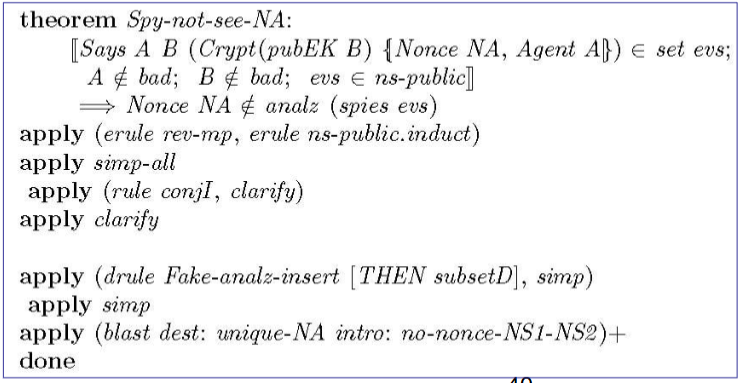
\includegraphics[width=0.7\linewidth]{Images/capitolo_5/esempio_teorema.png}
\end{figure}
Come notiamo in figura, per dimostrare il teorema effettuiamo una serie di passaggi logici tramite "applicazioni" di altri teoremi o lemmi precedentemente dimostrati.
